\documentclass[conference]{IEEEtran}
\usepackage{bm}
\usepackage{bbm}
\usepackage{amsmath}
\usepackage{amsthm}
\usepackage{algorithm,algorithmic}
\usepackage{url}
\usepackage{authblk}
\usepackage{amssymb}
\usepackage{mathtools}
\usepackage{graphicx}
\DeclarePairedDelimiter\norm{\lVert}{\rVert}
\DeclareMathOperator{\Var}{Var}
\newtheorem{definition}{Definition}
\newtheorem{theorem}{Theorem}
\newtheorem{lemma}{Lemma}
\newtheorem{remark}{Remark}
\newtheorem{corollary}{Corollary}
\DeclareMathOperator{\SSBM}{SSBM}
\DeclareMathOperator{\SDP}{SDP}
\DeclareMathOperator{\Tr}{Tr}
\DeclareMathOperator{\E}{\mathbb{E}}
\DeclareMathOperator{\diag}{diag}
\DeclareMathOperator{\dist}{dist}
\DeclareMathOperator{\Bern}{Bern}
\DeclareMathOperator{\Binom}{Binom}
\DeclareMathOperator{\KL}{KL}

\newcommand{\A}{\frac{a \log(n)}{n}}
\newcommand{\B}{\frac{b \log(n)}{n}}
\title{Exact Recovery in the Balanced Stochastic Block Model with Side Information}
\author[1]{\textbf{Jin Sima}}
\author[2]{\textbf{Feng Zhao}}
\author[3]{\textbf{Shao-Lun Huang}}
\affil[1]{\normalsize{Department of Electrical Engineering, California Institute of Technology, Pasadena 91125, CA, USA}}
\affil[2]{\normalsize{Department of Electronic Engineering,
		Tsinghua University, 
		Beijing, China 100084}}
\affil[3]{\normalsize{DSIT Research Center,
		Tsinghua-Berkeley Shenzhen Institute,
		Shenzhen, China 518055}}
	\allowdisplaybreaks[4]
\begin{document}
	\maketitle
	\begin{abstract}
		The role that side information plays in improving the exact recovery threshold in the stochastic block model (SBM) has been studied in many aspects. This paper studies 
		exact recovery in balanced binary symmetric stochastic block models with side information, given in the form of i.i.d. samples at each node. Compare to existing works, the balanced constraint in the SBM gives us two benefits. First, we derive a closed form sharp exact recovery threshold. Second, we present an efficient semi-definite programming (SDP) algorithm that achieves the optimal exact recovery threshold. Our SDP algorithm is a non-trivial generalization of the SDP algorithm for SBM without side information in the sense that our proof involves more detailed arguments.	
		% The role that side information plays in improving the exact recovery threshold in the stochastic block model (SBM) has been studied in many aspects. This paper studies 
		% 	exact recovery in balanced binary symmetric stochastic block models with side information, given in the form of i.i.d. samples at each node.
		% 	The balanced constraint in the SBM allows us to derive a sharp exact recovery threshold that is analytical. We also present an efficient semi-definite programming (SDP) algorithm that achieves the optimal exact recovery threshold. Our SDP algorithm is a non-trivial generalization of the SDP algorithm for SBM without side information in the sense that our proof involves more detailed arguments. Moreover, the SDP algorithm also applies to the binary SBM where the label of each node has a uniform distribution.
	\end{abstract}
	\section{Introduction}
	The stochastic block model (SBM) \cite{holland1983stochastic}, also known as the planted partition model, is a statistical model that admits clean theoretical analysis and efficient algorithms while capturing some of the key features exhibited in large data networks, such as social, biological, and computer networks \cite{abbe2015exact}. 
	The SBM describes a graph of $n$ nodes, partitioned into multiple communities. Each edge in the graph exists independently with a probability determined by the communities the two nodes on the edge belong to. The goal is to recover  the community each node belongs to, based on one instance of the graph edges. While there are several levels of recovery defined and studied (see \cite{Abbe17} for a comprehensive survey), in this paper we focus on the exact recovery, which aims to recover all the communities. 
	
	For exact recovery in the SBM, a more interesting regime is when the edge connecting probabilities are in order of $O(\frac{\log n}{n})$, in which circumstance there is a phase transition in the exact recovery condition. 
	The tight threshold on the exact recovery in this setting was not established until the work of \cite{abbe2015exact,mossel2016}, where efficient and optimal algorithms based on semi-definite programming (SDP) were also provided. 
	The results in \cite{abbe2015exact,mossel2016} were generalized in \cite{abbe2015community} where the sharp threshold for multiple comunities with asymmetric edge connecting probabilities is derived, and in \cite{Hajek16}, where optimal SDP algorithms for multiple communities and two communities with unequal community sizes are given.
	
	While the SBM focuses on graphical data only, it is natural to study the benefit of additional local data at the nodes, referred to as side information, to the exact recovery in the SBM. Such setting arises in applications where multi-modal data is observed. For example, in a social network, not only the interactions among people, but also the profile of each individual can be collected. It has been shown in many studies that side information such as node attributes or features \cite{zhang2016community,mossel2016local} can assist the community detection tasks. For exact recovery in the SBM with side information, the work of \cite{abbe17sideinfo} generalized \cite{abbe2015community} and derived a sharp threshold for exact recovery in the SBM with side information, given in the form of $\log n$ (in according with the order of the edge connecting probabilities) data samples at each node, drawn identically and independently  according to a probability distribution determined by the community the node belongs to. The communities are described by node labels, which are i.i.d. according to a probability distribution. 
	The threshold in \cite{abbe17sideinfo} holds for general cases and is expressed in the form of an optimization problem, to which no closed form solution can be found. The work of \cite{esmaeili2019exact,esmaeili2019community,saad2018community} considered more specific cases where side information is given as partial revealed labels and noisy labels.
	
	In this paper, we consider balanced binary symmetric SBM with side information in the form of i.i.d. node samples, drawn according to a distribution determined by the community the node belongs to. The balanced property in this paper means that the two communities in the graph have equal sizes. At the first glance, the setting in this paper might look like a special case of that in \cite{abbe17sideinfo}, where the each node belongs to any one of the two communities with probability $\frac{1}{2}$. 
	Yet, 
	the difference between the balanced assumption in this paper and the equal probability assumption in \cite{abbe17sideinfo},  which  also the contributions of this paper, is as follows. 
	
	
	First, while no closed form expression of the exact recovery threshold can be established in \cite{abbe17sideinfo} for  the binary symmetric SBM, in this paper, we derived a sharp and closed form threshold when balanced assumption is considered. Note that the result in \cite{abbe17sideinfo} does not imply our threshold. Our threshold indicates a separation between the side information and the graph data. Such separation provides an insight that the graph data and the side information can be designed and collected independently to achieve exact recovery. 
	Second, we proposed an SDP based algorithm that achieves the threshold with high probability, while an SDP algorithm is not available in \cite{abbe17sideinfo}. Note that the admissibility of an SDP algorithm normally requires a balanced assumption \cite{abbe2015exact},
	\cite{esmaeili2019community} or other assumptions that the community sizes are fixed \cite{Hajek16}. Our SDP algorithm is a generalization of the SDP in \cite{abbe2015exact} where side information is included. To this end, we added more linear constraints to the SDP problem and the proof is more involved.
	
	The paper is organized as follows. In Section 
	In Section \ref{s:model}, we introduce the model and present some definitions and lemmas needed throughout the paper. Section \ref{s:sharp} presents a sharp bound on exact recovery, which is one of the main results in this paper. In Section \ref{s:sdp}, we provide an SDP algorithm that achives the optimal threshold. Section \ref{s:conclusion} concludes the paper.
	
	
%	\newpage
%	In network analysis, community detection assigns discrete labels to each node of the graph based on the observation of graph edges.
%	In addition to edge information, extra node features are often available in real-world applications in the form of graph signal \cite{dong2020graph},
%	noisy labels \cite{mossel2016local}, or
%	feature vectors \cite{zhang2016community}. Combining the edge and node information, it is expected that better
%	accuracy can be achieved for community detection problems. Within this context, a central problem 
%	is to investigate the gain that extra information brings to the detection problem, compared to the case when only edge observation is available.
%	
%	% first paragraph: short intro to SBM and Ising model
%	To get theoretical insight into such a problem, it is often assumed that the graph is generated from a simple probabilistic model called Stochastic Block Model (SBM), in which the probability of edge existence is higher within the community than between different communities \cite{holland1983stochastic}. For the solely presence of SBM, the condition on exact recovery of community labels has been studied extensively and the phase transition property has been established \cite{abbe2015community, mossel2016}. For a special case of two community model,
%	the recovery condition is summarized as $\sqrt{a} - \sqrt{b} > \sqrt{2}$ when $a,b$ are parameters of SBM.
%	
%	With the presence of extra node information, the condition of exact recovery is improved
%	and generalized \cite{saad2018community, abbe17sideinfo}. However, previous study does not exactly quantify the contribution of side information and graph information. In contrast, this paper will fill the gap by considering a model of two-community SBM with extra node feature vectors. Our result generalizes
%	the exact recovery threshold to a condition $\gamma D_{1/2}(p_0 || p_1) + (\sqrt{a} - \sqrt{b})^2 > 2$
%	where the contribution of side information is coded in Renyi divergence.
%	
%	To achieve the exact recovery condition of SBM, semi-definite programming (SDP) is often utilized \cite{Hajek16}.
%	SDP relaxation can also be used for SBM with side information \cite{esmaeili2019exact}, and in this paper we show that a sub-optimal exact recovery condition
%	of our model is achievable by such method.
%	
%	This paper is organized as follows. In Section \ref{s:rw}, we review the previous works which are closely related with ours.
%	In Section \ref{s:model}, we introduce the model and present our main results.
%	Then the article concludes in Section \ref{s:conclusion} and
%	detailed proofs are provided in Section \ref{s:proof}.
%	
%	The following notations are used throughout this paper: 
%	the random undirected graph $G$ is written as $G(V,E)$ with vertex set $V$ and edge set $E$;
%	$V=\{1,\dots, n\} =: [n]$;
%	$\mathcal{X}$ is the alphabet
%	of the random variable $X$; $m$ is the number of samples generated at each node;
%	$\Bern(p)$ and $\Binom(n,p)$ represent Bernoulli
%	and Binomial distribution respectively; $f(n)=\omega(g(n))$(or $=o(g(n))$) means that $\lim_{n\to \infty} f(n) / g(n) = \infty $(or $=0$);
%	$\mathbbm{1}[A]$ is the indicator function for the event $A$; $W^n$ is the n-ary Cartesian power of the set $W$;
%	The Hamming distance of 
%	two $n$-dimensional vectors is written as $\dist(x,y):=\sum_{i=1}^n \mathbbm{1}[x_n\neq y_n]$ for $x,y\in \{\pm 1 \}^n$.
%	
%	\section{Related Works}\label{s:rw}
%	This work extends the model of two-community SBM considered in \cite{abbe2015community}.
%	Specifically, we assume the extra feature vectors of each node are independent samples, whose distribution depends on the label of the node.
%	This model has been studied in Section V-B of \cite{saad2018community}. However,
%	\cite{saad2018community} only got a weak conclusion, which says that the sample complexity of feature vectors
%	$m$ is required to be of order $O(\log n)$ for side information to take effects. In this paper, we obtain
%	a closed-form condition for exact recovery when $m=\gamma \log n$ for a positive constant $\gamma$.
%	
%	A general case of side information is studied
%	in \cite{abbe17sideinfo}. We emphasize that the model setting in Theorem 4 of \cite{abbe17sideinfo}
%	assumes that the node labels are independently generated  from $\Bern(\frac{1}{2})$ while the model
%	in this paper requires uniform distribution over the space $\sum_{i=1}^n Y_i = 0$ where $Y_i \in \{\pm 1 \}$ is the label of the $i$-th node.
%	Although these two settings are equivalent in
%	SBM model when $n$ is large, we observe that it differs when side information is available. Our assumption is easier to analyze due to some
%	symmetric property of node observations.
%	
%	Rényi divergence has been used in SBM in \cite{zhang2016} to characterize the weak recovery error bound. Both the dense and sparse graph are considered.
%	Within this paper, we use Rényi divergence to characterize
%	the contribution of side information to exact recovery error bound in these two cases.
	\section{Preliminaries}\label{s:model}
	A balanced binary symmetric SBM is defined by a random graph $Z=\{Z_{i,j}\}_{1\le i,j\le n}$ with $n$ nodes $\{1,\ldots,n\}$ and edges $\{Z_{i,j}\}_{1\le i,j\le n}$, where $Z_{i,j}=1$ if nodes $i$ and $j$ are connected with an edge and $Z_{i,j}=0$ otherwise. 
	Each node $i\in\{1,\ldots,n\}$ is associated with a label $Y_i\in \{\pm 1\}$ such that the label $Y=(Y_1,\ldots,Y_n)$ is uniformly distributed over the space $\{Y:\sum^n_{i=1}Y_i=0\}$. The edges $\{Z_{i,j}\}_{1\le i,j\le n}$ are independently distributed Bernouli random variables, where $Z_{i,j}=1$ with probability $p=a\frac{\log n}{n}$ for nodes $i,j$ with the same labels, i.e., $Y_i=Y_j$, and $Z_{i,j}=1$ with probability $q=b\frac{\log n}{n}$ if $Y_i\ne Y_j$. In this paper, it is assumed that $a>b$. 

	
	
	
	A balanced binary symmetric SBM with side information (SBMSI) is a generalization of the balanced SBM. In addition to the graph $Z$ and the labels $Y$, each node $i$ has $m=\gamma \log n$ data samples $X^i_{j}$, $i\in \{1,\ldots,n\}$, $j\in \{1,\ldots,m\}$, that are drawn identically and independently from distribution $P_0$ if $Y_i=1$ and from distribution $P_1$ if $Y_i=-1$. Note that the data samples $X^i_{j}$, $j\in \{1,\ldots,m\}$ are independent from $\{Z_{i,j}\}_{1\le i,j\le n}$ given the label $Y_i$ for any $i\in\{1,\ldots,n\}$. Hence, the joint probability distribution of $(\{Z_{i,j}\}_{1\le i,j\le n},\{X^i_{j}\}_{1\le i\le n,1\le j\le m})$ conditioned on $Y$ is
	\begin{align}\label{eq:lh}
		&P(x=\{x^i_{j}\}_{1\le i\le n,1\le j\le m},z=\{z_{i,j}\}_{1\le i,j\le n}| (y_1,\ldots,y_n)) \nonumber\\
		=& \prod_{1\le i,j\le n}P(z_{i,j}|y_i,y_j)\prod_{i=1}^n \prod_{j=1}^m P(x^i_j|y_i), 
	\end{align}
	where 
	\begin{equation*}
		P  (z_{i,j}=1|y_i,y_j) = \begin{cases}
			p & \text{if } y_i=y_j \\
			q & \text{if } y_i\ne y_j
		\end{cases},
	\end{equation*}
	and
	\begin{equation*}
		P(x^i_j|y_i) = \begin{cases}
			P_0(x^i_j) & Y_i = 1 \\
			P_1(x^i_j) & Y_i = -1
		\end{cases}
	\end{equation*}
	The conditional probability distribution $P(\{x^i_{j}\}_{1\le i\le n,1\le j\le m},\{z_{i,j}\}_{1\le i,j\le n}| y_1,\ldots,y_n)$ is determined by parameters $n$, $p$, $q$, $P_0$, and $P_1$. Hence, 
	the SBMSI is denoted as $SBMSI(n,p,q,P_0,P_1)$.
	In $SBMSI(n,p,q,P_0,P_1)$, the goal is to recover the unknown labels $Y$, given the graph $Z$ and the data samples $X$. In this paper, we consider exact recovery of $Y$, which is defined as follows.
	\begin{definition}[Exact Recovery for $SBMSI(n,p,q,P_0,P_1)$]
		Let
		$(Z=\{Z_{i,j}\}_{1\le i,j\le n},Y,X=\{X^i_{j}\}_{1\le i\le n,1\le j\le m})$ be a graph $Z$, node labels $Y$, and node data samples $X$ be drawn from the distribution defined by $SBMSI(n,p,q,P_0,P_1)$.
		Exact recovery is solvable if there exists an algorithm that takes $(Z,X)$ as inputs and outputs $\hat{Y}=\hat{Y}(Z,X)$ such that the error probability $P_e:=P(\hat{Y} \neq Y)$ goes to $0$ as $n$ increases.
	\end{definition}
	A key measure used throughout this paper is the Rényi divergence, defined by
	\begin{equation}
		D_{1/2}(P_0 || P_1) \triangleq -2\log(\sum_{x \in \mathcal{X}} \sqrt{P_0(x)P_1(x)} ),
	\end{equation}
	where $P_0$ and $P_1$ are the distributions defined in the balanced   $SBMSI(n,p,q,P_0,P_1)$.
	%The Rényi divergence characterizes the error exponent of a SSBM when the graph observation $Z$ is not  available and exact recovery of the labels $Y$ is done with only side information $X$. 
	The following property of the Rényi divergence will be needed in proving our main results. It can be proved by using the Lagrange multiplier.
	\begin{lemma}\label{lem:p0p12}
		Let $p_0, p_1$ be probability distribution functions defined over $\mathcal{X}$. The minimizer
		of $D(X||p_0) + D(X||p_1)$ for any discrete random variable $X$ is
		\begin{equation}\label{eq:p012}
			P(X=x)=\frac{\sqrt{p_0(x)p_1(x)}}{ \sum_{x\in \mathcal{X}} \sqrt{p_0(x) p_1(x)}}
		\end{equation}
		and the minimal value is
		$-2\log \sum_{x\in \mathcal{X}} \sqrt{p_0(x) p_1(x)}$.
	\end{lemma}
	\section{Sharp Threshold for Balanced SBMSI}\label{s:sharp}
	In this section we present a sharp closed form threshold for exact recovery in the balanced SBMSI.  %We first provide the threshold, that comes from
	%the phase transition in the exact recovery in SBMSI with sparse graph structure. 
	\begin{theorem}\label{thm:Pe}
		For a balanced $SBMSI(n,p=a\frac{\log n}{n},q=b\frac{\log n}{n},P_0,P_1)$, exact recovery is solvable if
		\begin{equation}\label{eq:positive_condition}
			\gamma D_{1/2}(P_0||P_1) + (\sqrt{a} - \sqrt{b})^2 > 2,
		\end{equation}
			in which case, the error probability
	\begin{equation*}
		P_e \leq (1+o(1)) n^{-\frac{1}{2}\left(\gamma D_{1/2}(p_0||p_1) + (\sqrt{a} - \sqrt{b})^2-2\right)},
	\end{equation*}
		and is not solvable if $\gamma D_{1/2}(p_0||p_1) + (\sqrt{a} - \sqrt{b})^2 < 2$, in which case, the error probability $P_e$ goes to $1$.
	\end{theorem}
	\begin{remark}
	Theorem \ref{thm:Pe} implies a separation of graph observation and side information, in the sense that the left part of \eqref{eq:positive_condition} is exactly the sum of the terms that appear in the exact recovery threshold in SBM  when there is graph observation only \cite{abbe2015exact} and when there is side information only, respectively. This separation is in contrast to the case in \cite{abbe17sideinfo}, where side information $X$ and graph observation $Z$ are coupled and a joint optimization in both $Z$ and $X$ with no closed form solution is needed. In Fig. \ref{fig:my_label} we show a comparison of our threshold and the one from \cite{abbe17sideinfo} when $P_0$ and $P_1$ are Bernouli random variables with probability $ 0.05$ and $0.5$, respectively and $\gamma=5$.  It can be seen that there is a slight difference between the results in \cite{abbe17sideinfo} and in this paper.		We note that when such difference is small, our threshold can be used as an approximation to the threshold in \cite{abbe17sideinfo}, which is easily computable and provides insight to design the system. For example, when the parameters $a$ and $b$ are fixed in the graph, one can easily find the number of samples $m=\gamma\log n$ needed to achieve a given exact recover error probability. 
	\end{remark}
	\begin{figure}
	    \centering
	    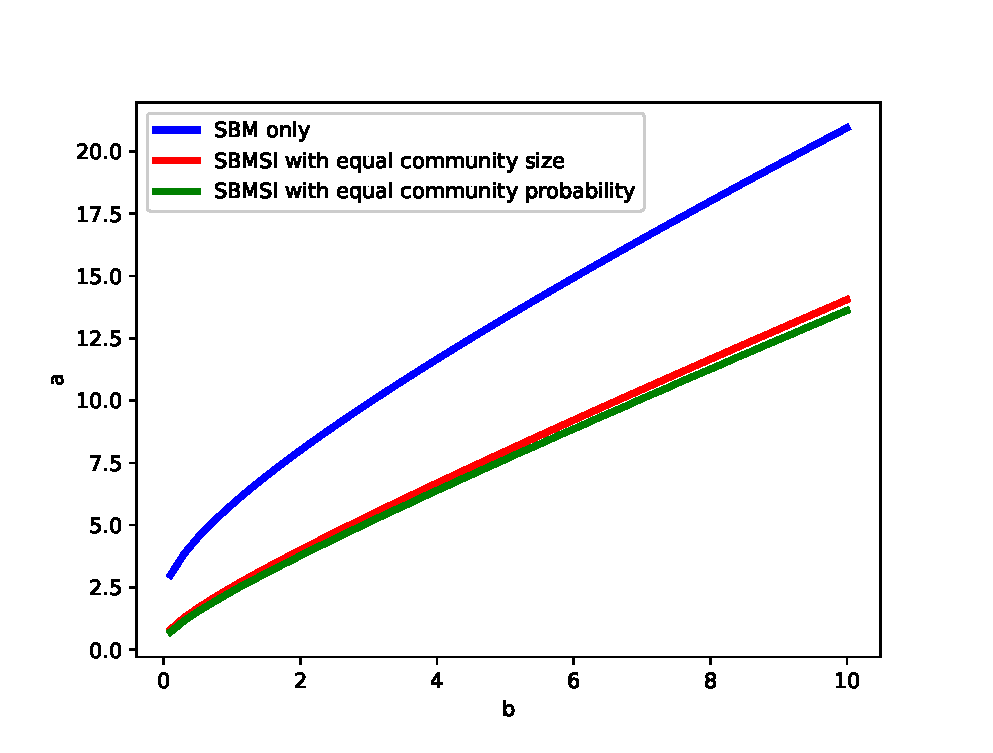
\includegraphics[width=0.4\textwidth]{comparison.eps}
	    \caption{Theoretical comparison of different thresholds with $P_0 \sim \Bern(0.05), P_1\sim \Bern(0.5), \gamma=5$. The blue, red, and green lines show results from \cite{abbe2015exact}, this paper, and \cite{abbe17sideinfo}, respectively.}
	    \label{fig:my_label}
	\end{figure}

	\subsection{Proof of Theorem \ref{thm:Pe}}
	%\begin{proof}[Proof of Theorem \ref{thm:Pe}]
%	The proof of Theorem \ref{thm:Pe} follows similar arguments to those in \cite{abbe2015exact}. We first show the first part of Theorem \ref{thm:Pe}, i.e., the achievability of exact recovery when \eqref{eq:positive_condition} holds. For any label $Y=(Y_1,\ldots,Y_n)$ satisfying $\sum^n_{i=1}Y_i=0$, let $A(Y)=\{i:Y_i=1\}$ and $B(Y)=\{i:Y_i=-1\}$ be the sets of nodes with labels $1$ and $-1$, respectively.  
%	Let $Y^*=(y^*_1,\ldots,y^*_n)$ be the true labels of the nodes. We prove that with high probability, $Y^*$ is the output of an MAP (maximum a posteriori probability) estimator, which is equivalent to an ML (maximum likelihood) estimator since $Y$ is uniformly distributed over the space $\{Y:\sum^n_{i=1}Y_i=0\}$.
%	Let $F_k$ be the event that there exists a labeling $Y'$ satisfying $|A(Y')\backslash A(Y)|=|B(Y')\backslash B(Y)|=k$. Then, by the union bound, it suffices to show that the probability $P(F_k)$ of the event $F_k$ is upper bounded by $o(\frac{1}{n})$ for anly $k\in\{1,\ldots,n\}$.
%	
%	Let $P_k$ be the maximum probability that 
%	the likelihood $P(X,X| (Y^*_1,\ldots,Y^*_n)$ is smaller than the likelihood $P(X,Z| (Y'_1,\ldots,Y'_n))$, 
%	over all labeling $Y'=(Y'_1,\ldots,Y'_n)$ satisfying $|A(Y')\backslash A(Y)|=|B(Y')\backslash B(Y)|=k$, where the likelihood $P(X,Z| (Y_1,\ldots,Y_n)$ is defined in \eqref{eq:lh}. Then by the union bound, we have that 
%	\begin{equation}\label{eq:FAk}
%		P(F_k) \leq \binom{n/2}{k}^2 P_k
%	\end{equation}
%	It remains to derive an upper bouond on $P_k$. 
%	According to \eqref{eq:lh}, $P_k$ is the probability that
%	\begin{align}\label{eq:ein}
%		&\sum^m_{j=1}(\sum_{i\in A(Y^*)\backslash A(Y')} \log \frac{P_1(X^i_{j})}{P_0(X^i_{j})}
%		+\sum_{i\in A(Y')\backslash A(Y^*)} \log \frac{P_0(X^i_{j})}{P_1(X^i_{j})})\nonumber\\
%		\ge & \log \frac{p(1-q)}{q(1-p)} (\sum_{i\in A(Y^*)\backslash A(Y'),j\in A(Y^*)\cap A(Y')}z_{i,j}\nonumber\\
%		&+\sum_{i\in A(Y')\backslash A(Y^*),j\in B(Y^*)\cap B(Y')}Z_{i,j}\nonumber\\
%		&-\sum_{i\in A(Y^*)\backslash A(Y'),j\in B(Y^*)\cap B(Y')}Z_{i,j}\nonumber\\
%		&-\sum_{i\in A(Y')\backslash A(Y^*),j\in A(Y^*)\cap A(Y')}Z_{i,j})
%	\end{align}
%	Note that the right hand side of \eqref{eq:lh} can be written as $\log \frac{p(1-q)}{q(1-p)}(Z_1-Z_2)$, where $Z_1\sim Binom(k(n-2k),\frac{a\log n}{n})$ and $Z_2\sim Binom(k(n-2k),\frac{b\log n}{n})$ 
%	follow binomial distributions, where a binomial distribution $Binom(s,r)$ is the probability distribution of the sum of $s$ independent Bernouli random variables, each equals $1$ with probability $r$.
%	The left hand side can be expressed as
%	\begin{align*}
%		\epsilon\triangleq&\log^{-1}( a /b)\cdot [\sum_{i\in A(Y^*)\backslash A(Y')}(D(P_{\widetilde{X}^i} || P_0) - D(p_{\widetilde{X}^i} || P_1)) \\
%		&+ \sum_{i\in A(Y')\backslash A(Y^*)}(D(p_{\widetilde{X}^i} || P_1) - D(p_{\widetilde{X}^i} || P_0))],
%	\end{align*}
%	where $P_{\widetilde{X}^i}$ is the empirical distribution of samples $\{x^i_j\}^m_{j=1}$ at node $i$. 
%	
	
	
	
%	\begin{proof}[Proof of Theorem \ref{thm:Pe}]
%		We start from \eqref{eq:ein}.
%		Since $m=\gamma \log n$, $\sum_{i=1}^{km} \log \frac{p_1(x_{1i})}{p_0(x_{1i})} \sim
%		-km D(p_0 || p_1)$, which is of order $O(\log n)$.
%		Let $\epsilon$ be defined as follows:
%		
%		
%		Then \eqref{eq:ein} is equivalent to
%		\begin{equation}\label{eq:zeps}
%			\sum_{i=1}^{k(n-2k)}(z'_{i} - z_{i}) \geq \epsilon \log n
%		\end{equation}
%		Using the type theory (11.1 of \cite{cover1999elements}), we can estimate the probability of the event $A_k$ given by \eqref{eq:zeps}.
%		\begin{align}
%			P(A_k) & =  \sum_{P^{(1)},P^{(2)}\in \mathcal{P}_{km}} Q_0^{km}(T(P^{(1)}))Q_1^{km}(T(P^{(2)}))\notag \\
%			& \cdot P(\sum_{i=1}^{k(n-2k)} (z'_{i} - z_{i} \geq \epsilon(P^{(1)}, P^{(2)})  \log n ))\label{eq:decomp} 
%		\end{align}
%		Then using Theorem 11.1.4 of \cite{cover1999elements} and Lemma \ref{lem:zxt} 
%		\begin{align*}
%			&P(A_k)  \leq \sum_{P \in P_n} \exp(-km (D(p_{\widetilde{X}_1} || p_0) + D(p_{\widetilde{X}_2} || p_1))) \\
%			& \cdot \exp(-\log n \frac{k(n-2k)}{n}\cdot (g(a, b, \frac{n}{k(n-2k)}\epsilon) + o(1))) \\
%			&\leq |\mathcal{P}_{km}|^2 \exp(-k\log n \cdot (\theta^*_k + o(1))) 
%		\end{align*}
%		where
%		\begin{align}
%			\theta^*_k &= \min_{\widetilde{X}_1,\widetilde{X}_2} \gamma (D(p_{\widetilde{X}_1}|| p_0) + D(p_{\widetilde{X}_2} || p_1)) \notag \\
%			&\quad + (1-\frac{2k}{n}) g(a,b, \frac{n}{k(n-2k)}\epsilon) \label{eq:theta_star}
%		\end{align}
%		
%		By Lemma \ref{lem:p0p12}, we can get
%		\begin{align}
%			\theta^*_k &\geq (1-\frac{2k}{n})(\sqrt{a} - \sqrt{b})^2
%			+ \frac{ \gamma}{2}\min (D(p_{\widetilde{X}_1}||p_0) + D(p_{\widetilde{X}_1}||p_1)) \notag \\
%			&+ \frac{ \gamma}{2}\min (D(p_{\widetilde{X}_2}||p_0) + D(p_{\widetilde{X}_2}||p_1))\notag \\
%			&=  (1-\frac{2k}{n})(\sqrt{a} - \sqrt{b})^2 - 2 \gamma\log(\sum_{x\in\mathcal{X}}\sqrt{p_0(x)p_1(x)}) 
%			\label{eq:theta_star_lower_bound}
%		\end{align}
%		Next, we show that the lower bound is achievable.
%		When the probability distribution of $\widetilde{X}_1, \widetilde{X}_2$ takes the form given by \eqref{eq:p012},
%		$\epsilon = 0$, and $\theta^*_k$ in \eqref{eq:theta_star} is exactly the lower bound \eqref{eq:theta_star_lower_bound}.
%		Since $\theta^*_k>0$,
%		and $|\mathcal{P}_{km}|\leq (km+1)^{|\mathcal{X}|} $, we have $P(A_k) \leq n^{-k(\theta^*_k+o(1))}$.
%		
%		Using the union bound, we can control $P(F_k)$ by
%		$$
%		P(F_k) \leq \binom{n/2}{k}^2 P(A_k)
%		$$
%		When $k \geq \frac{n}{\sqrt{\log n}}$, using Lemma 8 of \cite{feng2021},
%		$P(F_k)$ decreases exponentially. The error probability for $k < \frac{n}{\sqrt{\log n}}$
%		is analyzed using \eqref{eq:FAk}.
%		\begin{align*}
%			&P_e \leq (1+o(1))\sum_{k=1}^{\frac{n}{\sqrt{\log n}}} P(F_k) \leq (1+o(1)) \cdot \\
%			&\sum_{k=1}^{\frac{n}{\sqrt{\log n}}} \exp(k(-\mu \log n + \frac{2k}{n} \log n(\sqrt{a} - \sqrt{b})^2 - 2\log 2k + 2))
%		\end{align*}
%		where $\mu = (\sqrt{a} - \sqrt{b})^2-2 + \gamma D_{1/2}(p_0||p_1) > 0$.
%		Using the inequality
%		$$
%		\frac{2k}{n}(\sqrt{a} - \sqrt{b})^2\log n -2\log2k+2\leq \frac{\mu}{2} \log n
%		$$
%		for $1\leq k \leq \frac{n}{\sqrt{\log n}}$, we can obtain
%		\begin{align*}
%			P_e &\leq(1+o(1)) \sum_{k=1}^{\frac{n}{\sqrt{\log n}}} \exp(k(-\mu \log n/2)) \\
%			& =(1+o(1)) \frac{n^{-\mu / 2}}{1-n^{-\mu / 2}} = (1+o(1))n^{-\mu / 2}
%		\end{align*}
%		Therefore, \eqref{eq:PeMain} is established.
%		\newpage
		The achievability part can be proved by our SDP algorithm, the details of which will be given in  Section \ref{s:sdp}.
		In the following we show that exact recovery is not possible if $\gamma D_{1/2}(p_0||p_1) + (\sqrt{a} - \sqrt{b})^2 < 2$. Most part of the arguments follow a similar manner to those in \cite{abbe2015exact}. Those similar arguments are briefly stated due to space limitation. 
		
		Let $S_1$ and $S_2$ be the set of nodes with labels $1$ and $-1$, respectively. Let $H_1$ be a subset of $S_1$ of size $\frac{n}{\log^3 n}$. It was shown in \cite{abbe2015exact} that in the SBM, with probability at least $\frac{9}{10}$, no node in $H_1$ is connected to more than $\frac{\log n}{\log\log n}$ edges in $H_1$. Similarly, let $H_2$ be a subset of $S_2$ of size $\frac{n}{\log^3 n}$. Then, with high probability $H_2$ satisfies the same property as $H_1$ does. 
		
		For any $i_1\in H_1$ and $i_2\in H_2$, let $F(i_1,i_2)$ be the event that the likelihood $P(X,Z|(Y_1,\ldots,Y_n))$ (defined in \eqref{eq:lh}) with $Y_{i_1}=-1,Y_{i_2}=1$ is larger than the likelihood $P(X,Z|(Y_1,\ldots,Y_n))$ with $Y_{i_1}=1,Y_{i_2}=-1$, which results in  recovery failure because the maximum likelihood estimate is equivalent to maximum a posteriori probability estimate when $Y$ is uniformly distributed. For a node $i$ and a node set $S\subset\{1,\ldots,n\}, $let $E(i,S)$ be the number of edges between $i$ and nodes in $S$. Then, according to \eqref{eq:lh}, the event $F(i_1,i_2)$ is equivalent to  
		the following 
		\begin{align}
			&\sum_{j=1}^{m} \log \frac{P_1(x^{i_1}_{j})}{P_0(x^{i_1}_{j})}
			+\sum_{j=1}^{m} \log \frac{P_0(x^{i_2}_{j})}{P_1(x^{i_2}_{j})}\nonumber\\
			\ge &\log \frac{p(1-q)}{q(1-p)}(E(i_1, S_1 \backslash \{i_1\}) + E(i_2, S_2 \backslash \{i_2\})\nonumber\\
			&- E(i_1, S_2 \backslash \{i_2\}) - E(i_2, S_1 \backslash \{i_1\})) \label{eq:F1ij}.
		\end{align}
		By the definition and property of $H_1$ and $H_2$ mentioned above, the probability of \eqref{eq:F1ij} is lower bounded by the probability of
		\begin{align}
			&\sum_{j=1}^{m} \log \frac{P_1(x^{i_1}_{j})}{P_0(x^{i_1}_{j})}
			+\sum_{j=1}^{m} \log \frac{P_0(x^{i_2}_{j})}{P_1(x^{i_2}_{j})}\nonumber\\
			\ge &q\log \frac{p(1-q)}{q(1-p)}(2\frac{\log n}{\log\log n}+E(i_1, S_1 \backslash \{i_1\}) + E(i_2, S_2 \backslash \{i_2\})\nonumber\\
			&- E(i_1, S_2 \backslash \{i_2\}) - E(i_2, S_1 \backslash \{i_1\})) \label{eq:G1ij}.
		\end{align}
		with high probability. Let $G(i_1,i_2)$ be the event that \eqref{eq:G1ij} holds for any $i_1\in H_1$ and $i_2\in H_2$. In the next, we show that
		the probability of $G(i_1,i_)$ is lower bounded by $\frac{1}{n^{-2+\mu}}$ for some positive constant $\mu$. Then we have that 
		\begin{align}
			& P(\cap_{i_1\in S_1, i_2\in S_2} F^c(i_1,i_2)) = (1 - P(F(i_1,i_2)))^{|H_1|\cdot|H_2|} \nonumber\\
			& \le (1 - P(G(i_1,i_2)))^{|H_1|\cdot|H_2|}\nonumber\\
			& \leq (1-n^{-2+u})^{n^2/\log^6 n} \nonumber\\
			& \leq \exp(-n^{\mu+ o(1)}) \to 0, \label{eq:boundg}
		\end{align}
		where $F^c(i_1,i_2)$ is the event that $F(i_1,i_2)$ does not occur. Eq. \eqref{eq:boundg} implies that with high probability $F(i_1,i_2)$ occurs for some $i_1\in S_1$ and $i_2\in S_2$, and hence the failure occurs.
		
		Note that the right hand side of \eqref{eq:G1ij} can be written as $\log \frac{p(1-q)}{q(1-p)}(Z_1-Z_2+o(\log n))$, where $Z_1\sim Binom(n-2,\frac{a\log n}{n})$ and $Z_2\sim Binom(n-2,\frac{b\log n}{n})$ 
		follow binomial distributions, where a binomial distribution $Binom(s,r)$ is the probability distribution of the sum of $s$ independent Bernouli random variables, each equals $1$ with probability $r$.
		The left hand side can be expressed as
		\begin{align*}
			\epsilon\triangleq&m\log^{-1}( a /b)\cdot [(D(P_{\widetilde{X}^{i_1}} || P_0) - D(P_{\widetilde{X}^{i_1}} || P_1)) \\
			&+(D(P_{\widetilde{X}^{i_2}} || P_1) - D(P_{\widetilde{X}^{i_2}} || P_0))],
		\end{align*}
		where $P_{\widetilde{X}^i}$ is the empirical distribution of samples $\{x^i_j\}^m_{j=1}$ at node $i$. Let $P_{\widetilde{X}^{i_1}}$ and $P_{\widetilde{X}^{i_2}}$ follow the distribution specified in \eqref{eq:p012}. Then we have that $\epsilon =0$. Using Sanov's theorem and Lemma 4 from \cite{abbe2015exact}, we have that
		\begin{align*}
			&P(G_1(i,j))\\
			\geq &\frac{1}{(m+1)^{2|\mathcal{X}|}} \exp(-m(D(p_{\widetilde{X}_1} || p_0) + D(p_{\widetilde{X}_2} || p_1)) \\
			&\cdot\exp(- (\sqrt{a} - \sqrt{b})^2\log n+o(\log n) ) \\
			& = \exp(-\log n (\gamma D_{1/2}(P_0||P_1) + (\sqrt{a} - \sqrt{b})^2+ o(1))),
		\end{align*}
		where $\mathcal{X}$ is the alphabet of distributions $P_0$ and $P_1$.
		Since $\gamma D_{1/2}(P_0||P_1) + (\sqrt{a} - \sqrt{b})^2<2$, we have that $P(G_1(i,j))\ge n^{-2+\mu}$ for some positive constant $\mu$.
%	\end{proof}
	

	
	\section{SDP Relaxation}\label{s:sdp}
	In this section, we propose a semi-definite programming based relaxation to find the maximum likelihood estimate of the labels $Y$. Note that
	the ML estimate of the labels $Y$ is NP-hard. 
	Our SDP algorithm finds the true label $Y^*$ with probability approaching $1$, if
	$\gamma D_{1/2}(p_0||p_1) + (\sqrt{a} - \sqrt{b})^2 > 2$.
	The SDP problem can be solved using various efficient iterative schemes.
	
	Let $S_+(Y)$ and $S_-(Y)$ be the sets of nodes with label $1$ and $-1$, respectively, given $Y$.
	According to \eqref{eq:lh}, the log likelihood of $Y$ is given by
	\begin{align}\label{eq:loglh}
		&\sum^m_{j=1}[\sum_{i\in S_+(Y)} \log P_1(X^i_{j})+\sum_{i\in S_-(Y)} \log P_0(X^i_{j})]\nonumber\\
		&+\sum_{i,j\in S_+(Y),i<j}[z_{i,j}\log p+(1-z_{i,j})\log (1-p)]\nonumber\\
		&+\sum_{i,j\in S_-(Y),i<j}[z_{i,j}\log p+(1-z_{i,j})\log (1-p)]
		\nonumber\\
		&+\sum_{i\in S_+(Y),j\in S_-(Y)}[z_{i,j}\log q+(1-z_{i,j})\log (1-q)].
	\end{align}
	It can be verified that maximizing \eqref{eq:loglh} over $Y\in\{\pm\}^n$ is equivalent to the following optimization problem
	\begin{align}
		\max_{x}\, & h^T v + \frac{1}{2}v^T B v \notag \\
		s.t.\, & \mathbbm{1}_n^T v = 0 \text{ and } v_i \in \{\pm 1 \} \label{eq:matrix_mle}
	\end{align}
	where $h$ is an n-dimensional vector with entry $h_i = \frac{1}{\log \frac{p(1-q)}{q(1-p)}}\sum_{j=1}^m \log \frac{P_0(x^i_{j})}{P_1(x^i_{j})}$ for $i\in\{1,\ldots,n\}$ and the $n\times n $ matrix $B$ is defined as
	\begin{equation}
		B_{ij} = \begin{cases}
			1, & \text{if $i$ is concected to $j$}, \\
			-1,& \text{else.}
		\end{cases}
	\end{equation}  
	for $i,j\in\{1,\ldots,n\}$.
	%However, we find that
	%the maximal solution is unchanged when $\kappa$ takes other values as long as $\kappa > b\frac{\log %n}{n}$.
	
	Let $v^*$ be the optimal solution to \eqref{eq:matrix_mle} and $V=(1,v^*)(1,v^*)^T$, where $(1,v^*)$ is a $(n+1)$-dimensional  vector obtained by concatenating $1$ and $v^*$.
	Then, the optimal value of \eqref{eq:matrix_mle} equals $\frac{1}{2}Tr(\widetilde{B}V)$, where
	\begin{equation}\label{eq:B_lambda_def}
		\widetilde{B} = \begin{pmatrix} 0 & h^T  \\ h  & B \end{pmatrix}.
	\end{equation}
	We wish to show that $V$ is the unique optimal solution to the following problem.
	\begin{align}
		\max\, Tr(\tilde{B}V)  &\notag\\
		s.t.\, V_{ii} &= 1, \notag\\
		V &\succeq 0, \notag\\
		\sum_{j=1,j\neq i}^{n+1} (V_{ij} + V_{ji})& = 0,~\forall i\in\{1,\ldots,n\}. \label{eq:sdp}
	\end{align}
	Note that here we use $n+1$ constrains in the last line of \eqref{eq:sdp} to describe the balanced property of the labels. This is important in deriving the optimality and uniqueness of $V$, which will be proved in the following theorem. The theorem shows that our SDP relaxation achieves exact recovery with high probability, if the threshold is met.
	%When $m=0$ and $\kappa=1$,
	%the SDP is exactly the one Abbe considered in \cite{abbe2015exact}.
	%When $m=0$ and $\kappa=\frac{a-b}{\log a/b}\frac{\log n}{n}$, the SDP is
	%the same as the one in Theorem 3 of \cite{Hajek16}.
	% The theoretical guarantee for the relaxation form in \eqref{eq:sdp} is summarized
	% in the following theorem:
	\begin{theorem}\label{thm:sdp}
		If $\gamma D_{1/2}(p_0||p_1)  + (\sqrt{a} - \sqrt{b})^2 > 2$, then with high probability, the optimal solution
		$V^*$ to \eqref{eq:sdp} is unique and given by $(1,y^*)(1,y^*)^T$, where $y^*$ is the true labeling of the nodes.
	\end{theorem}
	\begin{proof}[Proof of Theorem \ref{thm:sdp}]
	Consider the dual problem of \eqref{eq:sdp}
	\begin{align}
		\min &\sum_{i=1}^{n+1} a_i \nonumber\\\label{eq:dual}
		s.t. &\, \diag\{a_1, \dots, a_{n+1}\} + \Xi - \widetilde{B} \succeq 0, 
	\end{align}
	where the $(n+1)\times (n+1)$ symmetric matrix $\Xi$ is defined as 
	\begin{equation}
		\Xi_{ij} = \begin{cases}
			0, & i=j \\
			\lambda_i + \lambda_j, & i\neq j
		\end{cases},
	\end{equation}
	WLOG, let $g=(1,\ldots,1,-1,\ldots,-1)$ be the true labels of the nodes, i.e., the first and second half of the nodes are labeled by $1$ and $-1$, respectively. As similarly mentioned in \cite{abbe2015exact},
	the optimality and uniqueness of the solution $(1,g)(1,g)^T$ to \eqref{eq:sdp} is guaranteed by the following conditions: 
	\begin{enumerate}
		\item[(a)] $(1,g)(1,g)^T$ is a feasible solution to the primal problem \eqref{eq:matrix_mle}.
		\item[(b)] There exists a feasible solution $(a_1,\ldots,a_{n+1},$ $\lambda_1,\ldots,\lambda_{n+1})$to \eqref{eq:dual}, such that $\sum_{i=1}^{n+1} a_i=Tr((1,g)(1,g)^T\widetilde{B})$.
		\item[(c)] $(\diag\{a_1, \dots, a_{n+1}\} + \Xi - \widetilde{B})(1,g)=0$.
		\item[(d)] The second smallest eigenvalue of $\diag\{a_1, \dots, a_{n+1}\} + \Xi - \widetilde{B}$ is greater than $0$. 
	\end{enumerate}
	Condition (a) holds by definition. It suffices to choose $(a_1,\ldots,a_{n+1},\lambda_1,\ldots,\lambda_{n+1})$ that satisfies conditions (b), (c) and (d).
	Let $\mu=\frac{1}{n}\mathbbm{1}_n^T h$ and $\lambda = -u/n$. Specify $(a_1,\ldots,a_{n+1},$ $\lambda_1,\ldots,\lambda_{n+1})$ as follows
	$$\lambda_1=\mu, \text{ and }\lambda_{i+1}=g_i\lambda + \lambda,~i\in\{1,\ldots,n\}$$
	Then, from condition (c) we have that
	\begin{align}
		a_1 &= h^T g - n\lambda \nonumber\\
		a_{i+1} & = (h_i +\lambda)g_i + \lambda + \frac{1}{2}\diag\{Bgg^T\}, i = 1, \dots, n
	\end{align}
	It can be verified that $\sum_{i=1}^{n+1} a_i = 2h^Tg +\frac{1}{2} g^T B g$, and hence condition (b) holds.
	Hence it suffices to prove that
	\begin{align}
		&\diag(y) + \Xi - \widetilde{B} \nonumber\\
		=& \begin{pmatrix} h^T (g+\frac{1}{n}\mathbbm{1}_n) & -h^T +(\mu + \lambda)\mathbbm{1}_n^T + \lambda g^T\\
			-h+(\mu + \lambda )\mathbbm{1}_n + \lambda g& \Xi_n \end{pmatrix}
		\succeq 0, 
	\end{align}
	where
	\begin{align}\label{eq:Xi_n}
		\Xi_n =&\diag(hg^T + Agg^T -\lambda \mathbbm{1}_ng^T)  \nonumber\\
		&+ (\frac{1}{2} +2\lambda) J_n -\lambda I_n - A + 2\lambda \Xi',
	\end{align}
	$\mathbbm{1}_n$ is the all 1's vector, $J_n$ is the all 1's matrix, and $I_n$ is the identity matrix. The matrix $A=(B+J_n-I_n)/2$ is the adjacency matrix of the graph.
	The matrix $\Xi'$ is given by $\Xi'_{ij}=g_i + g_j$.
	
	In the following we show that $\Xi_n$ is positive definite. Then according to condition (c) and the
	Cauchy's Interlace Theorem, condition (d) holds.
	Then, the proof is done.
	
	We show that $x^T \Xi_n x>0$ for any vector $x \in \mathbb{R}^n$ satisfying $\norm{x}=1$. Decompose $x$ as $x=\frac{\beta}{\sqrt{n}} g
	+ \sqrt{1-\beta^2} g^{\perp}$, where $g^Tg^{\perp}=0, \beta \in [0,1]$, and $\norm{g^{\perp}}=1$. Then, we have that 
	\begin{align}
		x^T \Xi_n x = \frac{\beta^2}{n} g^T \Xi_n g  &
		+		\frac{\beta}{\sqrt{n}}\sqrt{1-\beta^2} g^T \Xi_n g^{\perp}
		\nonumber\\\label{eq:xax}
		&+
		(1-\beta^2)(g^{\perp})^T \Xi_n g^{\perp}. 
	\end{align}
	In the next we derive lower bounds to the three terms in the right hand side of \eqref{eq:xax}.
	For the first term, we have that
	\begin{align*}
		g^T \Xi_n g = g^T(h -\lambda I_n) -\lambda  = g^T h-\lambda
	\end{align*}
	Since $\mathbb{E}[g_ih_i]$ is a positive number of order $O(n\log n)$ and $\lambda$ has order at most $O(\log n)$,
	by Sanov's theorem or Chernoff bound, the probability 
	$P(g^T h < 0)$ decreases exponentially in $n$. Hence, with high probability, the first term $g^T \Xi_n g$ is positive.
	
	For the second term, let $\tilde{h}=(g^T \Xi)^T
	=(n-1)\lambda\mathbbm{1}_n+h-\lambda g$, then
	$g^T \Xi_n g^{\perp} = \tilde{h}^T g^{\perp} \geq -\norm{\tilde{h}-\frac{1}{n}(\tilde{h}^Tg)g}$, where the  norm $\norm{\tilde{h}-\frac{1}{n}(\tilde{h}^Tg)g}$ satisfies
	\begin{align*}
		\norm{\tilde{h}-\frac{1}{n}(\tilde{h}^Tg)g}^2
		=\norm{\tilde{h}}^2 - \frac{1}{n}(\tilde{h}^Tg)^2.
	\end{align*}
	Let $\hat{g}_1 = \frac{1}{2}(g + \mathbbm{1}_n)$ and $\hat{g}_2 = \frac{1}{2}(-g +\mathbbm{1}_n)$.
	Using the fact that $\tilde{h}^T\mathbbm{1}_n=\mu$, we have 
	\begin{align*} 
		&\frac{\norm{\tilde{h}}^2}{n} - (\frac{1}{n}\tilde{h}^Tg)^2\\
		&=\frac{\norm{\tilde{h}}^2}{n} - 2\frac{(\tilde{h}^T \hat{g}_1)^2}{n^2} - 2\frac{(\tilde{h}^T \hat{g}_2)^2}{n^2} + \frac{(\tilde{h}^T\mathbbm{1}_n)^2}{n^2} \\
		&=2\frac{ \sum_{i<j,i,j\in S_1} (\tilde{h}_i - \tilde{h}_j)^2 + \sum_{i<j,i,j\in S_2} (\tilde{h}_i - \tilde{h}_j)^2 }{n^2}+ \frac{\mu^2}{n^2}\\
		& = I_1 + I_2 + \frac{\mu^2}{n^2}.
	\end{align*}
	where $I_j=\frac{\sum_{i\in S_j} h_i^2}{n} - 2\frac{(h^T \hat{g}_j)^2}{n^2}$ for $j\in\{1,2\}$,  and $S_1$ and $S_2$ denotes the sets of nodes with label $1$ and
	$-1$, respectively. Denote $\mathbb{E}[h_i]=m D_j, \Var[h_i]=m \bar{D}_j, \mathbb{E}[h_i^2]=\Var[h_i]+\mathbb{E}^2[h_i]=m \bar{D}_j+m^2 D^2_j, \Var[h_i^2] \leq m^4 \bar{C}_j$ for $i\in S_j$ and $j\in\{1,2\}$. Then
	$D_j, C_j,j\in\{1,2\}$ are constants.
	Using Chebyshev's inequality, we have that
	\begin{align*}
		P(\Big| \frac{\sum_{i\in S_j} h_i^2}{n} - \frac{1}{2}(m \bar{D}_j + m^2D_j^2) \Big| \geq \log n) & \leq \frac{m^4 \bar{C}_j}{2n\log^2 n} \\
		P(\Big| \frac{h^T \hat{g}_j}{n} - \frac{m}{2}D_j\Big| \geq \log^{-1} n) & \leq \frac{m \log^{2} n\bar{D}_j}{2n}
	\end{align*}
	for $j\in\{1,2\}$. Hence, with probability $1-n^{1-o(1)}$, 
	\begin{align*}
		I_j \leq& \frac{1}{2}m\bar{D}_j + \frac{1}{2}m^2 D_j^2 + \log n - 2(\frac{1}{2}m D_j - \log^{-1} n)^2 \\
		=& O(\log n)
	\end{align*}
	for $j\in\{1,2\}$.
	Therefore, we have that
	$$
	\frac{1}{\sqrt{n}} g^T \Xi_n g^{\perp} \geq -\sqrt{\frac{\norm{\tilde{h}}^2}{n} - (\frac{1}{n}\tilde{h}^Tg)^2} = O(\sqrt{\log n})
	$$
	
	
	
	
	
	
	
	
	For the last term $(g^{\perp})^T \Xi_n g^{\perp}$, by \eqref{eq:Xi_n} and the fact that $(g^{\perp})^Tg=0$, we have that
	\begin{align*}
		&(g^{\perp})^T \Xi_n g^{\perp} \\
		=& (g^{\perp})^T \diag( -\lambda \mathbbm{1}_ng^T+hg^T + Agg^T) g^{\perp} + p -\lambda \\
		&+ \frac{1}{2}(1-p-q+2\lambda)(g^{\perp})^TJ_n g^{\perp}
		-(g^{\perp})^T(A-\mathbb{E}[A])g^{\perp},
	\end{align*}
	where we use the fact that $\mathbb{E}[A] = \frac{p-q}{2}gg^T + \frac{p+q}{2}J_n - pI_n$. Note that $p,q,$ and $\lambda$ are $o(1)$ terms and that $(g^{\perp})^TJ_n g^{\perp}\ge 0$. 
	By Theorem 5.2 of \cite{lei2015consistency},
	with probability $1-n^{-r}$, $\lambda_{\max}(A-\mathbb{E}[A]) \leq c\sqrt{\log n}$ for some positive constant $r$ and $c$. Hence, we have that
	\begin{align}\label{eq:lastterm}
		(g^{\perp})^T \Xi_n g^{\perp} \geq \min\{(-\lambda + h_i) g_i + g_i (Ag)_i \} - c \sqrt{\log n}
	\end{align}
	% The error probability is then bounded by
	% \begin{align*}
	% P(\Xi_{ii} \leq c\sqrt{\log n}, \forall 1\leq i \leq n)
	% \end{align*}
	We now show that with high probability,
	\begin{align}\label{eq:nodei}
		(-\lambda + h_i) g_i + g_i (Ag)_i  - c \sqrt{\log n}\ge 0
	\end{align}
	for $i\in\{1,\ldots,n\}$. For $g_i=1$,
	the term $(Ag)_i$ can be written as 
	$\log (Z_1-Z_2)$, where $Z_1\sim Binom(n-1,\frac{a\log n}{n})$
	and $Z_2\sim Binom(n-1,\frac{b\log n}{n})$ 
	follow binomial distributions. The term $h_ig_i=\gamma \frac{D(P_{\widetilde{X}_i} || P_1) - D(P_{\widetilde{X}_i} || P_0) }{\log a /b}$, where $P_{\widetilde{X}_i}$ is the empirical distribution of samples $\{X^i_j\}^m_{j=1}$ at node $i$. Then, we have the following lemma, which is a slight generalization of Lemma 8 in \cite{abbe2015exact} and can be proved using Chernoff bound.
	\begin{lemma}\label{lem:zxt}
		Suppose $m > n, Z \sim \Binom(m, \frac{b\log n}{n}), X\sim \Binom(m, \frac{a\log n}{n})$.
		For $ t \geq \frac{m}{n}(b - a)$, we have
		\begin{equation}\label{eq:estimation}
			P(Z - X \geq t \log n) \leq \exp(-\frac{m}{n}\log n \cdot ( g(a, b, \frac{n}{m}t) + O(\frac{\log n}{n})))
		\end{equation}
		where $g(a,b,\epsilon)$ is defined as
		\begin{equation}\label{eq:gab}
			g(a,b,\epsilon) = a + b - \sqrt{\epsilon^2 + 4ab} + \epsilon \log \frac{\epsilon + \sqrt{\epsilon^2 + 4ab}}{2b}
		\end{equation}
	\end{lemma}
	According to Lemma \ref{lem:zxt} and Sanov's theorem, the probability that \eqref{eq:nodei} does not hold is upper bounded by
	$n^{-\theta^*_i + o(1)}$ where
	\begin{align}
		\theta^*_i &= \min_{\widetilde{X}_1} \gamma D(p_{\widetilde{X}_1}|| p_0)+ \frac{1}{2} g(a,b, 2\epsilon) \label{eq:theta_star2},\mbox{ and} \nonumber\\
		\epsilon &= \gamma \frac{D(P_{\widetilde{X}_1} || P_1) - D(P_{\widetilde{X}_1} || P_0) }{\log a /b}
	\end{align}
	Since $\frac{\partial^2 g(a,b,\epsilon)}{\partial \epsilon^2} =\frac{1}{\sqrt{4ab+\epsilon^2}}> 0$, we have that
	\begin{equation}\label{eq:g_linear}
		g(a,b,\epsilon) \geq  (\sqrt{a} - \sqrt{b})^2 + \frac{\epsilon}{2}\log \frac{a}{b}. 
	\end{equation}
	Then, by Lemma \ref{lem:p0p12},
	\begin{align*}
		\theta^*_1 \geq \frac{1}{2}((\sqrt{a}-\sqrt{b})^2+\gamma \frac{P_{\widetilde{X}_1} || P_1) - D(P_{\widetilde{X}_1} || P_0)}{2} \\
		\geq \frac{1}{2}((\sqrt{a}-\sqrt{b})^2+\gamma D_{1/2}(P_0||P_1)),
	\end{align*}
	where the equality holds when $P_{\widetilde{X}_1}$ is given by \eqref{eq:p012}. 
	Similar error probability can be obtained when $g_i=-1$. Finally,
	by using the union bound, we conclude that the probability that $(g^{\perp})^T \Xi_n g^{\perp}\le 0$ is upper bounded by $n^{1-\theta_1^*+o(1)}$, and Theorem \ref{thm:sdp} holds.
\end{proof}
	% , and Theorem \ref{thm:sdp} gives a quantification of its theoretical
	% performance. For observations from binary symmetric channel, the result is
	% \begin{corollary}
	% 	Suppose $X_{ij}$ is the output of $Y_i$ from a binary symmetric channel with crossover probability
	% 	$p^*$. $P(\hat{Y}_{\SDP} \neq  Y) = o(1)$ as long as
	% 	\begin{equation}
	% 	-2\log(2\sqrt{p^*(1-p^*)}) + (\sqrt{a} - \sqrt{b})^2>2
	% 	\end{equation}
	% \end{corollary}
% 	\section{Experiment Result}
% 	The plot \ref{fig:my_label} shows that the empirical probability of successful recovery of the SDP algorithm 
% 	for the SBM with side information. We fix $n=300$ and the number of trials to be 20. The number of samples is chosen as $m=10$ for $\Bern(0.2)$ versus $\Bern(0.8)$. Then
% 	at each trial and for fixed $a$ and $b$, we check how many times each method succeeds. Dividing
% 	by the number of trials, we obtain the empirical probability of success with respect to
% 	the exact recovery metric. In blue, we plot the curve corresponding to the threshold $\sqrt{a}-\sqrt{b}=\sqrt{2}$ while in red we draw the curve corresponding to the threshold $\gamma D_{1/2}(p_0||p_1)  + (\sqrt{a} - \sqrt{b})^2 > 2$. 
% 	\begin{figure}
% 	    \centering
% 	    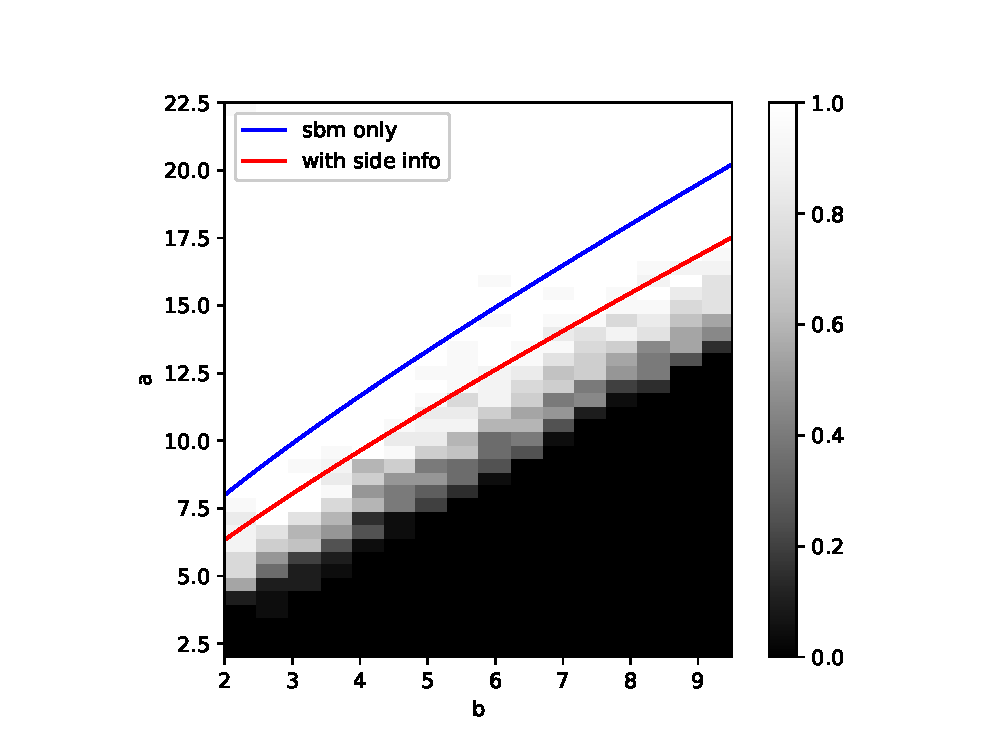
\includegraphics[width=0.5\textwidth]{fig.eps}
% 	    \caption{Comparison of different thresholds and with empirical recovery result by SDP}
% 	    \label{fig:my_label}
% 	\end{figure}

	\section{Conclusion}\label{s:conclusion}In this paper, we obtained a sharp close-form exact recovery condition for a balanced two-community symetric SBM with side information. %This condition
	%shows that the detection error can be %characterized by a separation of Rényi divergence and the parameters of SBM. To control the recovery error within a given level,
	Our result provides insight on the number of node samples to achieve exact recovery. We also proposed an Semidefinite programming based algorithm to achieve the threshold with high probability.
	\bibliographystyle{IEEEtran}
	\bibliography{exportlist}
\end{document}